\chapter{Methology}
\section{Market Design Descriptions}

- vielleicht noch einen allgemeine aussage wie szenarien in den verschieden Marktmodellen zu interpretieren sind.
.. oder ich beschreibe zuerst die verschiedenen märkte und dann die erstellung der dafür nötigen Daten.

\subsection{RL}
Der aFFr Markt in deutschland trennt sich in 2 Teile auf. Zum einen in den Regelleistungsmarkt und zum anderen in den Regelarbeitsmarkt.
Am Regelleistungsmarkt wird die bereitstellung von positiver oder negativer Regelleistung für ein 4 Stunden Zeitfenster am nächsten Tag geboten.
Auktionsschluss ist jeweils um 9 Uhr am Vortag.
Die Abrechnung erfolgt in [(Euro/MW)/h] der bezahlte Preis entspricht dabei dem eigenem Gebotspreis ("Pay-as-bid"-Verfahren).
	[https://www.next-kraftwerke.de/wissen/day-ahead-handel]
Bei bezugschlagtem Regelleistungsgebot muss auch für den selben Zeitraum am Regelarbeitsmarkt Gebote abgegeben werden werden.
\todo{eventuell raus lassen oder halt in vereinfachungsassumptions mit rein}
Die Mindestgebotsmenge beträgt 1 MW und zur Teilnahme ist eine Präquailifikation notwendig.

\subsection{DA}
Die erneuerbare Energien anlage wird am Day-Ahead Markt vermarktet. Hier werden Gebote für 1h Fenster am folgetag getätigt.
Die Auktion schließt um 12 am Vortag. Die Mindestmenge beträgt 0.1 MWh. Es werden Gebote zwischen -500 Euro und 3000 Euro aktzeptiert.
Die Abrechnung erfolgt in [Euro/MWh] und bezahlt wird im "Pay-as-cleared" Verfahren.
Das heißt alle bekommen den Preis des am höchsten noch bezugschlagtem Teilnehmers.

\subsection{RA}
Am sekundären Regelarbeitsmarkt wird auf 15 Minuten Fenster Geboten. Auktionsschluss ist jeweils 25 Minuten vor Begin des 15 Minuten Blocks.
Jeder vorqualifizierte Teilnehmer darf an diesem Markt mit bieten, egal ob ein zuschlag am Regelleistungsmarkt erfolgt ist oder nicht.
Wurde ein Regelleistungsmarktgebot bezugschlagt so muss auch auf das entsprechende Zeitfenster am Regelarbeitsmarkt geboten werden.
Bezahlt wird jeweils nur die tatsächlich erbrachte Leistung. Der Abbruf der Leistung erfolgt anhand der Merit-Order Liste, vom billigsten zum teuersten Anbieter.
Mit einem hohem angebotenen Regelarbeitspreis sinkt so die wahrscheinlichkeit für den Abruf der angebotenen Regelarbeit.
Dies ist ein Pay-as-cleared Market sprich alle Teilnehmer bekommen den Preis des letzten bezugschlagtem Teilnehmers.
Seit dem Beitritt Deutschlands zum PICASSO Netzwerk entspricht der Grenzpreis dem CBMP \cite{50hertzamprionTENNETTRANSNETBW.}.
\todo{ref}
\todo{mindestmenge?}

\section{General model explanation}

- profit maximierender ansatz\\
- reihenfolge der Entscheidungen\\
- wann klärt sich welche szenario unsicherheit auf\\

Ziel des Modells ist es auf möglichst einfache Weise eine Vermearktungsoptimierugn eines batterie speichers in kombination mit einem windpark vor zu nehmen.
Generell gibt es verschiedenste Möglichkeiten dies zu modellieren. Der Batteriespeicher wird am sekundären Regelleistungs und Regelarbeitsmarkt vermarktet.
Der Windpark wird am Day-Ahead-Markt angeboten. Wichtig hierbei ist es alle 3 Märkte miteinander zu verbinden ohne eine zu hohe komplexität zu benötigen die die Berechenbarkeit einschränkt.
Besonders wichtig ist dies zum Beispiel beim Batteriespeicher. Der aktuelle Ladestatus viertelstündlich neu berechnet. Selbst bei nur 2 möglichen Szenarien
wären das $ 2^{96} = 79228162514264337593543950336$ mögliche Batteriespeicher Zustände am Ende des Tages. Wenn man beachtet das die Planung immer für den Folgetag erfolgt
müsste man sogar $2^{182} = 6,13* 10^{54}$ mögliche Batteriespeicher Zustände beachten bevor man wieder Planungssicherheit hat.
\todo{den part nochmal nachdenken}
Da dies offensichtlich nicht mehr berechenbar ist muss man von perfekter Vorraussicht ausgehen und so nur einen Batteriespeicherweg berechnen.
Oder Bestimmte vorgänge innerhalb der Zeitkurve approimieren.
\todo{den part mit den speicherzuständen eventuell in die Modelierungsansatz Diskussion}

Lösungsansätze für dieses und andere Probleme sind im Abschnitt [] zu finden
\todo{abshcnitt eränzen}
Weiterhin ist zu beachten des sich der Windpark und der Batteriespeicher einen gemeinsamen Anschlusspunkt teilen, so ist die maximale Leistung beider begrenzt.

Es folgt eine Diskussion verschiedener Modellansätze. Anschließend werden die Einzelmodelle der verschiedenen Märkte betrachtet und zum schluss zusammen geführt.\\
-------------------------------------\\
\todo{aussortieren was noch mit oben rein soll}
Zur Analyse des vorliegenden Problems wurde ein Model in GAMS erstellt.
Ziel des Models war es auf möglichst geringem Rechenaufwand einen Batteriespeicher zu optimieren der mit
einer Analage zur produktion erneuerbarer energien kombiniert wurde. Dabei sollte vermmieden werden
auf sehr detailierte Zeitreihenvorhersagen, weil sehr aufwendig, angewiesen zu sein. Es sollten aber auch
Grundannahmen wie perfekte Vorraussicht vermieden werden um realistische Planungsentscheidungen ab zu bilden.

(Zur Vereinfachung werden zuerst alle Formeln für nur einen Zeitschritt aufgestellt. Am Ende wird die Zeitvariable entsprechend hinzugefügt.)
\todo{ausführliche Erklärung stochastische Programmierung}
\\
Das grundlegende Modell stellt einen Energiespeicher da, der am Regelleistungsmarkt, Day Ahead Markt und Regelarbeitsmarkt vermarktet werden kann.
Der darraus resultierende Profit soll maximiert werden. Für jede Teilentscheidung/Markt existiert ein eigenes Modell. So kann, für jedes Teilmodell,
vermieden werden die anschließenden Marktergebnisse (Zuschlag oder Ablehnung) zu integrieren. Dies ist wichtig, da anderen Falls der
Algorithmus allwissend wäre und nur perfekte Gebote errechnen würde. Die Ergebnisse eines jeden Teilmodells werden immer an das nachfolgende
Modell übergeben und erst an dieser Stelle ausgewertet. Jedes Teilmodell ermittelt Mengengebote zu bestimmten Preisen. Die verschiedenen Preise
werden durch verschiedene Szenarien abgebildet. Jedem Szenario ist eine bestimmte Wahrscheinlichkeit zugeordnet.
(Die Preis-Wahrscheinlichkeits-Kombinationen der verschiedenen Szenarien wurden vorher exogen mittels SARIMA-Analyse ermittelt.)
Ein Gebot stellt sich dann wie folgt dar:\\
---------------------------------\\

- modeldesign erklären
-> verschiedene designoptionen dann "design optionen"/alternativen/erklärung?!? part erklären
normalerweise liegt die logik in den daten und ich lasse den solver die logik in den daten erkennen.
wenn ich aber keinen realistischen vorcast daten habe muss ich die logik in das programm schon selber legen.

das wesentliche meiner

- anschluss punkt

- kombination aus park und batterie

\subsection{Modellierungansätze}
- eventuell in Konzepte umbenennen und ganz allgemein über verschiedene konzepte sprechen\\

Verschiedene Modellierungsansätze erfordern unterschiedliche zu grunde liegende Datensätze und anders herum.
So erfordert zum Beispiel ein stochastische model, welches eine optimierung über mehrere unsichere mögliche Szenarien vornimmt,
einen Datensatz der diese verschiedenen Szenarien abbildet. Bei der direkten verwendung historischer Daten benötigt man ein model,
welches  von einer perfekten Vorhersage ausgeht und so nur eine Datenreihe berücksichtigt.

Im folgenden werden verschiedene Ansätze bezüglich Model und Daten besprochen.

\subsubsection{Modelansätze Marktdesigns}

Ein möglicher Modelierungsansatz ist der der dem Model die perfekte Vorhersage unterstellt, hier werden historische
Daten eingespeist und anschließend die Ergebnisse
unter dieser Prämisse betrachtet. So werden dann die perfekten Ergebnisse mit einem abgeschätzen Prozentsatz herunterskaliert um zu einem
realistisch erzielbaren ergebnis zu kommen. Der Vorteil dieser Methode in unserem Fall läge in der einfachen Komplexität. Da man immer
genau weiß was eintritt muss auch nur ein einzelner Zeitstrahl verfolgt werden.
Der Nachteil liegt ganz klar darin das man bei der Betrachtung der Ergebnisse eventuell auf falsche Strategien schließt.
So müssen in  unserem Fall Entscheidungen getroffen werden mit unsicherer Zukunft Szenarien.
So kann es sein das zum Beispiel die Anschlusskapazität es nicht zulässt zugleich am DA-Markt und am RA- zu bieten.
\todo{abkürzungen} Bei perfekter Vorraussicht weiß ich genau welche entscheidung bei gegeben Daten die richtige ist auch wenn
der Unterschied zwischen den beiden Entscheidungen nur marginal ist.
Dies ist dann aber nur eine Einzelfallentscheidung, in realität kann es aber sein, dass eine andere strategie, über mehrere Fälle hinweg sich
als vorteilhaft herausstellt.
\todo{verweis wissenschaftliche arbeit und appendix für umsetzung}
So lassen sich mit diesem Ansatz gut Einzelfall entscheidungen treffen aber nicht gut auf eine allgemeine Strategie schließen.
Um eine Allgemeinere Strategie ableiten zu können bieten sich stochastische programmieransätze an. Diese bestimmen optimale Entscheidungen
unter betrachtung  mehrerer möglicher unsicherer Zukunftszenarien. So wird im Model eine entscheidungsvariable mit mehreren szenarien und deren
eintrittswahscheinlichkeiten kombiniert um so auf eine best mögliche Entscheidung unter Unsicherheit zu schließen.
So lassen sich einfacher optimalere allgemein gültige Strategien ableiten, allerdings ist hier die Erstellung der dafür notwendigen Daten wesentlich
schwieriger. So braucht man verschiedene Datensätze die die verschiedenen Szenarien präsentieren und muss diese Datensätze auch mit eintrittswahrscheinlichkeiten bewerten.
Im folgenden werden mehrere Ansätze diskutiert wie man dies für Zeitreihen-Datensätze macht \todo{abschnitt ergänzen}.
Außerdem müssen müssen oft vereinfachende Annahmen getroffen werden um die Modelkomplexität zu reduzieren.
Besonders wichtig ist dies zum Beispiel beim Batteriespeicher. In unserem Model wird der aktuelle Ladestatus des Batteriespeichers viertelstündlich neu berechnet. Selbst bei nur 2 möglichen betrachteten Szenarien
müsste man $ 2^{96} = 79228162514264337593543950336$ mögliche Batteriespeicher Zustände am Ende des Tages betrachten. Wenn man beachtet das die Planung immer für den Folgetag erfolgt
müsste man sogar $2^{182} = 6,13* 10^{54}$ mögliche Batteriespeicher Zustände beachten bevor man wieder Planungssicherheit hat. Deswegen werden erfolgt eine Betrachtung verschiedener Vereinfachungen in Kapitel []
\todo{den part nochmal nachdenken}\\
\todo{abschnitt ergänzen}\\

In Summe sind die Vorteile eine stochastischem Ansätzes größer, vor allem um die hier vorliegende Forschungsfrage nach allgemein güiltigen Strategien
zu beantworten.


Zur erstellung von optimalen allgemeinen strategien \\

\subsubsection{Modellierung von Zeitreihen}
Um auf gute allgemeine Strategien schließen zu können braucht es gute Daten. Falsche daten würden auch zu falschen Ergebnissen/Strategien führen.
Dabei gibt es verschiedene Ansätze diese Zeitreihendaten zu erstellen. Es folgt zuerst ein Überblick über die realwelt Daten um einen besseren eindruck
davon zu bekommen was wir probieren nach zu armen / vorherzusagen bzw. über welche wesentlichen eigenschaften die verschiedenen Marktdaten verfügen
Dazu werden die verschiedenen Marktdaten statischtisch dargestellt.
Anschließend werden verschiedene Analysemethoden diskutiert, kombiniert und angewandt.
In diesem Abschnitt werden verschiedene Methoden zur Erstellung von Zeitreihen diskutiert.
\subsubsection{Data Overview}
\textbf{RL}\\
Im ersten Fenster der übersicht [\ref{fig:Overview Average Negativ Capacity Price}] sind der Realmarktdaten von 2023 für den negativen Kapazitätsmarktpreis zu sehen.
Darunter ist der Trend und die Saisonalität abgebildtet.

\begin{figure}[!h]
	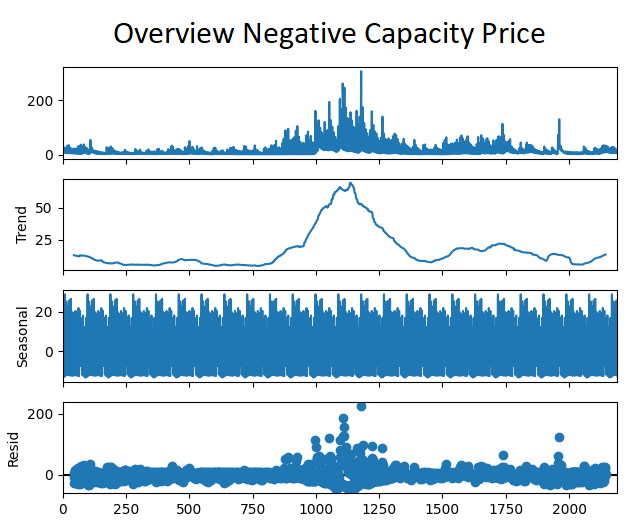
\includegraphics[width=1\linewidth]{pictures/capacityData_overview.png}
	\caption{Total Average Negativ Capacity Price}
	\label{fig:Overview Average Negativ Capacity Price}
\end{figure}

Bei einer genaueren Untersuchung der Saisonalität zeigt siche ein täglicher und ein leichter Wöchentlicher rythmus in den Daten.
Da es sich um Daten handelt die sich auf 4h-Blöcke beziehen sind alle 6 Lags als ein Tag zu interpretieren.
Abbildung \ref{fig:Autocorrelation Negative Capacity Price - 5 Days} zeigt dabei eine klaren täglichen rythmus in den Daten.

\todo{price in titel ergänzen}
\begin{figure}[!h]
	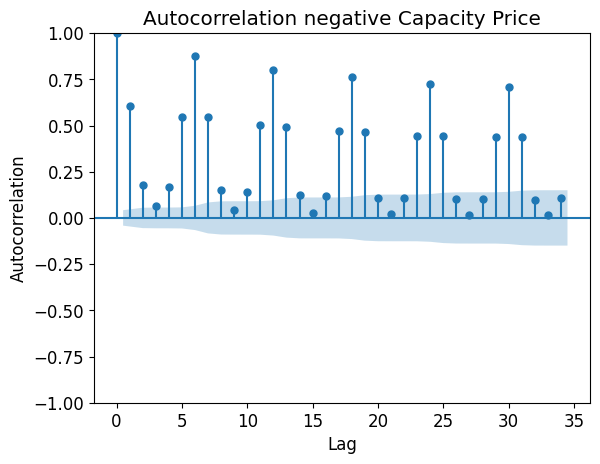
\includegraphics[width=1\linewidth]{pictures/Autocorrelation negative Capacity Price.png}
	\caption{Autocorrelation Negative Capacity Price - 5 Days}
	\label{fig:Autocorrelation Negative Capacity Price - 5 Days}
\end{figure}

Und Abbildung \ref{fig:AutocorrNegCap4Weeks} lässt zudem einen leichten wöchentlichen Zyklus erkennen.
\begin{figure}[!h]
	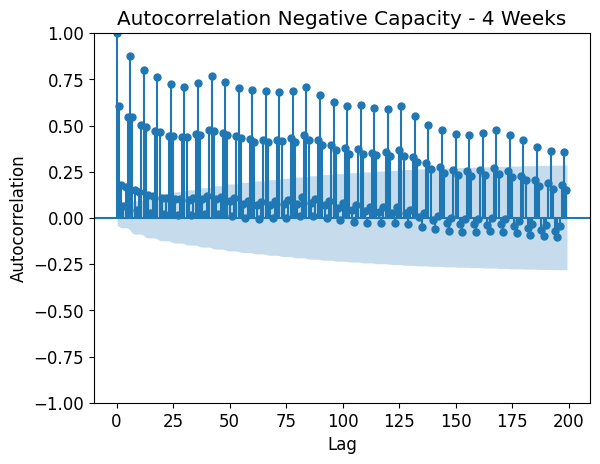
\includegraphics[width=1\linewidth]{pictures/Autocorrelation Negative Capacity - 4 Weeks.png}
	\caption{Autocorrelation Negative Capacity Price - 4 Weeks}
	\label{fig:AutocorrNegCap4Weeks}
\end{figure}

Die Preise zu den positiven Kapazitätwerten verhalten sich ähnlich wie die negativen Kapazitätswerte.

Zur anaylse und Zeitreihenvorhersage dieser Daten bieten sich nun, aufgrund der starken autocorrelation verschiedene statistische methoden an.
Dabei stellt sich besonders die ARIMA methode heraus. Diese beruht auf autoregression und ist somit besonders gut für zeitreihen mit starker
autorkorrelation geeignet. Um auch die Saisonalen effekte gut abbilden zu können gibt es eine Variante the ARIMA methode die SARIMA methode.

Ein ausführlicher Test der SARIMA methode, und der dafür notwendigen Tests befindet sich in Appendix \todo{verweis einfügen}. Dabei hat sich gezeigt, das die SARIMA methode schwächen mit der
komplexität in sehr langen Zeitreihen hat. So stieg die Rechenzeit expotential an und langfriste vorhersagen zeigten eine klare verzerrung hinsichtlich des letzten Trends.
Da wir aber kurzfristig ähnliche Jahresverläufe erwarten ist diese verzerrung folgend dem Trend am Jahresende nicht sinnvoll.
Außerdem ist die SARIMA analyse dafür ausgelegt Zeitreihendaten mit nur einer saisonalität zu erstellen. Für multiple Saisonalitäten wären aufwendige
manuelle anpassungen nötig. Ein Algorithmus der diese Nachteile vermeidet fußt auf den vorher genannten Konzepten und nennt sich TBATS.
TBATS is acronym for Trigonometric seasonality Box-Cox transformation ARMA errors Trend Seasonal components. Dieser Algorithmus von SKTIME erlaubt eine
einfachere Zeitreihenvorhersage bei gegebener multipler Saisonalität \cite{.05.04.2025}. \todo{appendix verweis}

Die somit vorhergsagte Zeitreihe ähnelt sehr der realen Zeitreihe. zu Beachten ist das die hier zu sehende Zeitreihe die Zeitreihe mit der höchsten Wahrscheinlichkeit ist.
So liegen 50\% der möglichen betrachteten Werte darüber und 50\% darunter. Wenn wir mit hilfe des vortrainierten predictors mehrere Szenarien/Zeitreihen
erstellen wollen so führt die inherente steigende ungewissheit mit steigenden Zeitabstand zu einer größerem intervall in dem die Daten liegen.
Das macht inhaltlich sinn und mag für viele anwendungsfälle sinnvoll sein, wir gehen aber davon aus das die mittlere vorhersage nicht an genauigkeit verliert
und wollen daraus szenarien generieren. Zu diesem Zweck wird die wahrscheinlichste/mittlere zeitreihenvorhersage genommen und manuel nach oben und nach unten
um bestimmte Prozentsäte hoch bzw. herunterskaliert. Die so erstellten Preisvorhersagen werden dann mit den realen Preisen verglichen und berechnet zu wievielen
Prozent mit der skalierten Zeitreihe ein Gebotszuschlag erfolgt wäre.

- hier eventuell noch rein das wenige daten ein hohes rauschen erzeugen
- wobei zuviele daten ein overfitting verursachen können


\begin{figure}[!h]
	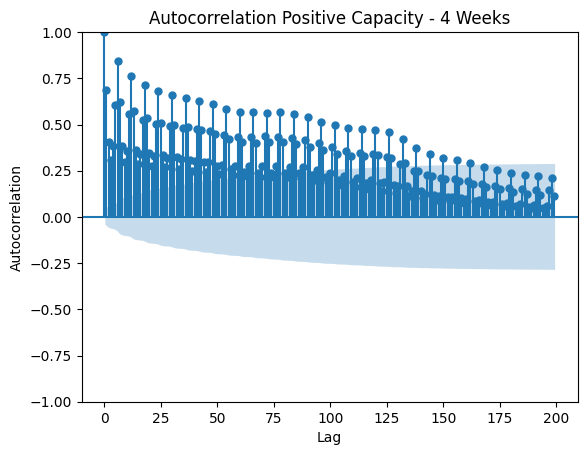
\includegraphics[width=1\linewidth]{pictures/autocorrelation_posCap_4weeks.png}
	\caption{Total Average Positive Capacity Price}
	\label{fig:Autocorrelation Positive Capacity  Price}
\end{figure}


\textbf{DA}\\
Die Day-Ahead Markt Preise sind zwar Variabel unterliegen aber einem Täglichem wie Wöchentlichen Rythmus.
Im Jahresverlauf sind nur allgemeine Trends ablesbar wie Abbildung \ref{fig:overviewDAprices} zeigt.
\begin{figure}[!h]
	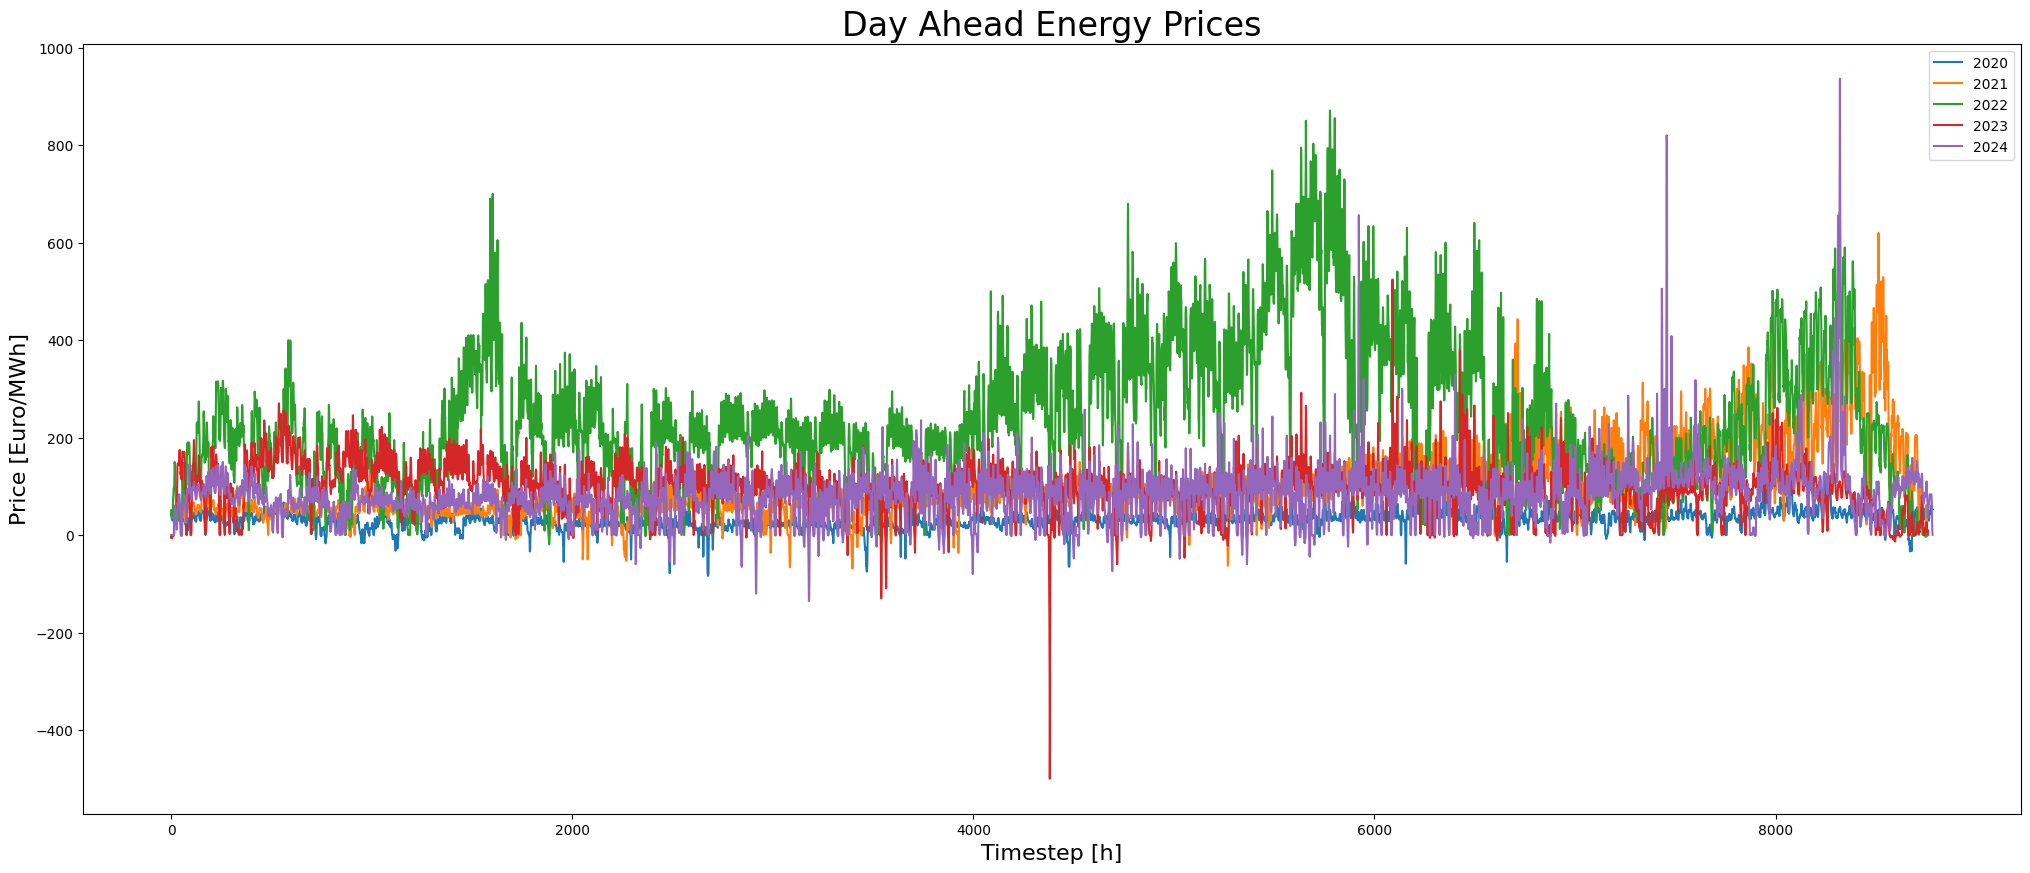
\includegraphics[width=1\linewidth]{pictures/overviewDAprices_year.png}
	\caption{Overview DA prices}
	\label{fig:overviewDAprices}
\end{figure}
Die außergewöhnliche Kurvenbewegung im Jahr 2022 ist mit dem Angriffskrieg Russlands gegen die Ukraine zu erklären
und den daraus folgenden Turbulenzen am Gas Markt.

Da es sich beim DA Markt um einen pay-as-cleared markt handelt (alle bekommen den Preis des am höchsten bezugschlagtem Teilnehmers)
und wir als Produzent erneurbarer Energien mit sehr geringen Opperationalen Kosten zu tun haben ist es für das model nur wichtig ob
wir am markt teilnehmen und welcher clearing price zu erwarten ist.

wie and Grafik \ref{fig:meanDA2020} bis \ref{fig:stdDA2024}      zu entnehmen ist zeigt der clearing price einen täglichen und wöchentlich  rythmus.
Das Nivau verändert sich zwar lässt sich aber gut verhersagen. Aufgrund des Marktdesigns brauchen wir auch nur einen erwarteten clearing price
da wir in der Realität ein 0-Preis Gebot abgeben können und somit sogut wie sicher bezuschlagt werden.
Der Erwartete Preis wird für unser Model als Mittelwert der Jahre 2020 bis 2024 ohne das Jahr 2022 kalkuliert. So erhalten die
Saisonale Struktur in den Daten und gleichen Ausreißer nach oben sowie nach unten aus. So ergibt sich je nach Tageszeit, Wochentag und Jahresverlauf ein zuverlässig
zu erwartender clearing-price.

\begin{figure}[h!]
	\centering
	\begin{minipage}{0.49\textwidth}
		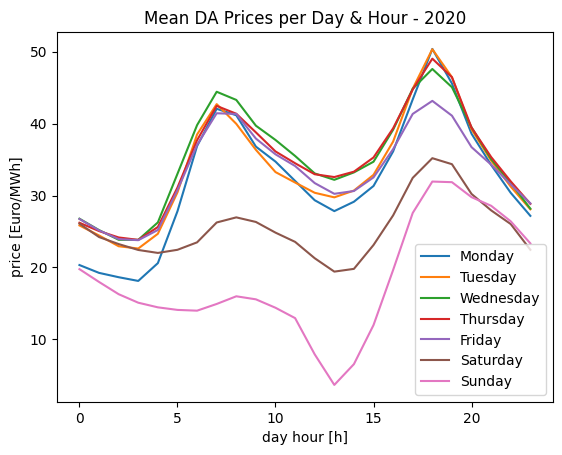
\includegraphics[width=1\linewidth]{pictures/DA/Mean DA Prices per Day and Hour - 2020.png}
		\subcaption{Mean DA-Price }
		\label{fig:meanDA2020}
	\end{minipage} \hfill
	\begin{minipage}{0.49\textwidth}
		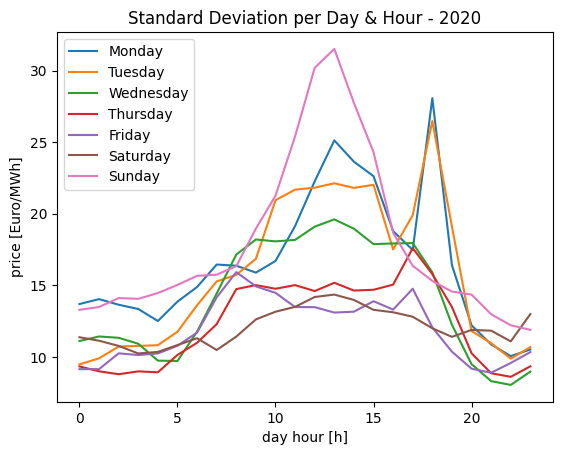
\includegraphics[width=1\linewidth]{pictures/DA/Standard Deviation per Day and Hour - 2020.png}
		\subcaption{Standard Deviation DA-Price}
		\label{fig:stdDA2020}
	\end{minipage}
	\caption{Daily and hourly DA-Data - 2020 }
\end{figure}

\begin{figure}[h!]
	\centering
	\begin{minipage}{0.49\textwidth}
		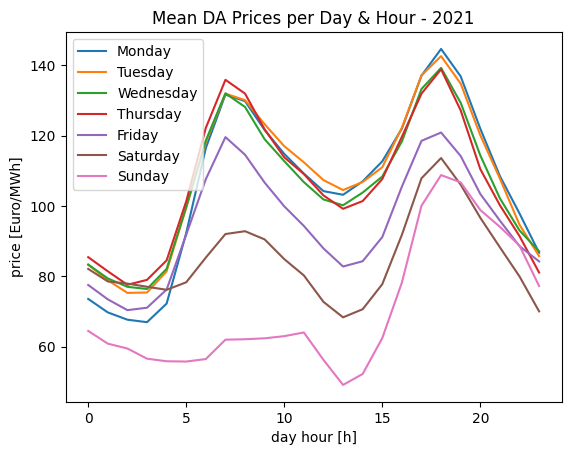
\includegraphics[width=1\linewidth]{pictures/DA/Mean DA Prices per Day and Hour - 2021.png}
		\subcaption{Mean DA-Price }
		\label{fig:meanDA2021}
	\end{minipage} \hfill
	\begin{minipage}{0.49\textwidth}
		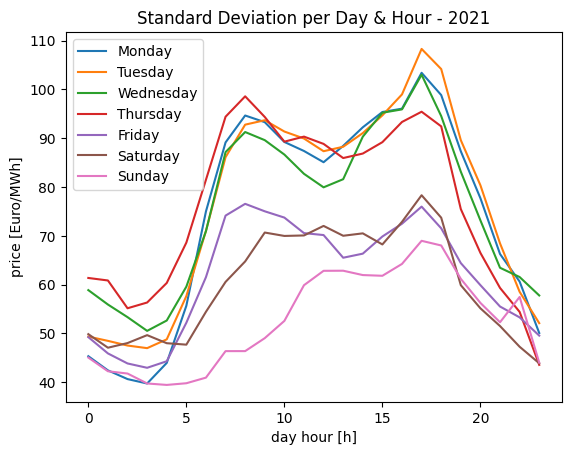
\includegraphics[width=1\linewidth]{pictures/DA/Standard Deviation per Day and Hour - 2021.png}
		\subcaption{Standard Deviation DA-Price}
		\label{fig:stdDA2021}
	\end{minipage}
	\caption{Daily and hourly DA-Data - 2021 }
\end{figure}

\begin{figure}[h!]
	\centering
	\begin{minipage}{0.49\textwidth}
		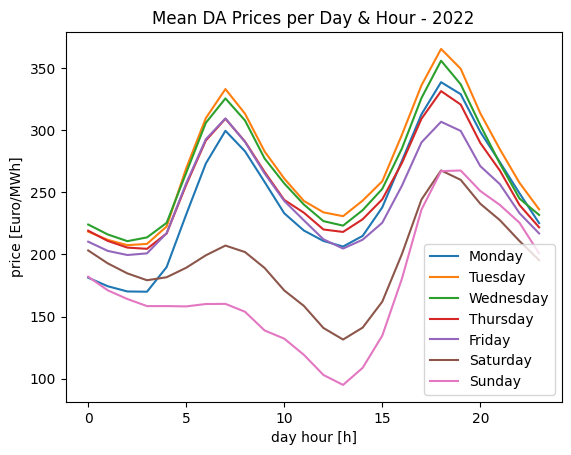
\includegraphics[width=1\linewidth]{pictures/DA/Mean DA Prices per Day and Hour - 2022.png}
		\subcaption{Mean DA-Price }
		\label{fig:meanDA2022}
	\end{minipage} \hfill
	\begin{minipage}{0.49\textwidth}
		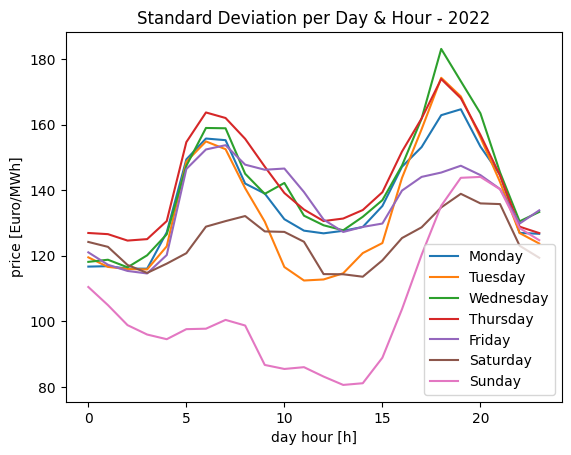
\includegraphics[width=1\linewidth]{pictures/DA/Standard Deviation per Day and Hour - 2022.png}
		\subcaption{Standard Deviation DA-Price}
		\label{fig:stdDA2022}
	\end{minipage}
	\caption{Daily and hourly DA-Data - 2022 }
\end{figure}

\begin{figure}[h!]
	\centering
	\begin{minipage}{0.49\textwidth}
		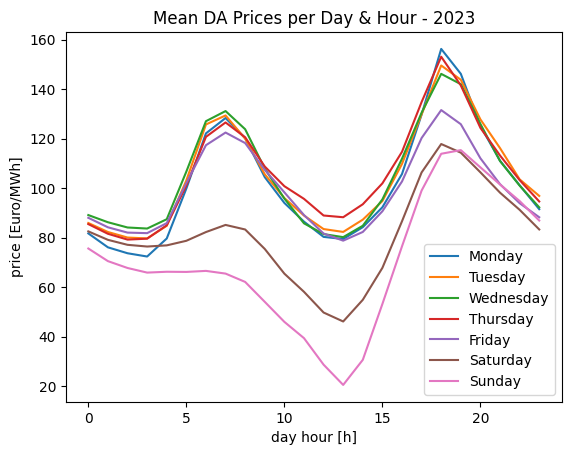
\includegraphics[width=1\linewidth]{pictures/DA/Mean DA Prices per Day and Hour - 2023.png}
		\subcaption{Mean DA-Price }
		\label{fig:meanDA2023}
	\end{minipage} \hfill
	\begin{minipage}{0.49\textwidth}
		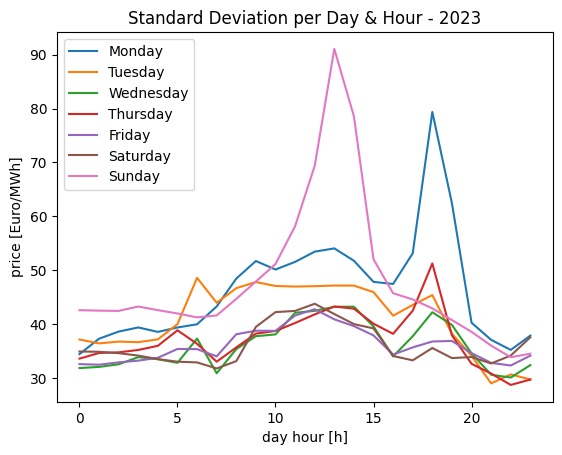
\includegraphics[width=1\linewidth]{pictures/DA/Standard Deviation per Day and Hour - 2023.png}
		\subcaption{Standard Deviation DA-Price}
		\label{fig:stdDA2023}
	\end{minipage}
	\caption{Daily and hourly DA-Data - 2023 }
\end{figure}

\begin{figure}[h!]
	\centering
	\begin{minipage}{0.49\textwidth}
		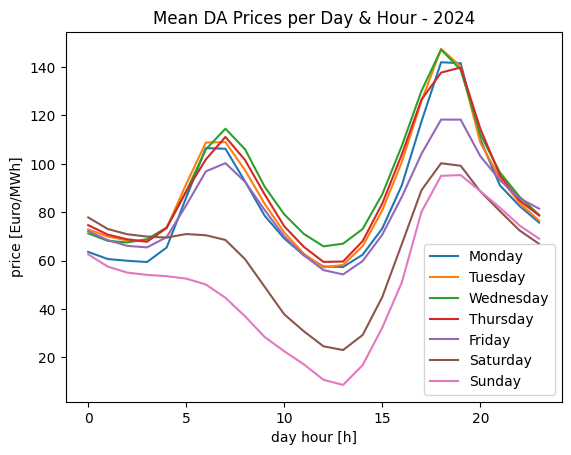
\includegraphics[width=1\linewidth]{pictures/DA/Mean DA Prices per Day and Hour - 2024.png}
		\subcaption{Mean DA-Price }
		\label{fig:meanDA2024}
	\end{minipage} \hfill
	\begin{minipage}{0.49\textwidth}
		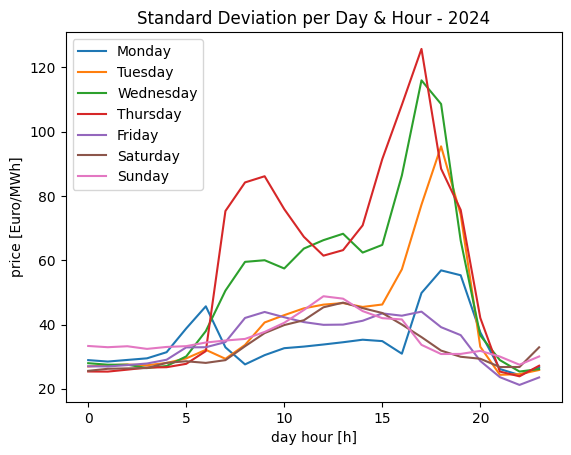
\includegraphics[width=1\linewidth]{pictures/DA/Standard Deviation per Day and Hour - 2024.png}
		\subcaption{Standard Deviation DA-Price}
		\label{fig:stdDA2024}
	\end{minipage}
	\caption{Daily and hourly DA-Data - 2024 }
\end{figure}


\textbf{RA}\\
Die RA unterliegen einer sehr hohen Variabilität und lassen sich nur sehr schwer statistisch vorherzusagen. So
verfügen sie nur über eine sehr schwache autocorrelation mit nur ganz leichtem wöchentlichem rythmus \ref{fig:Autocorrelation Positive Energy Price}.

hier ist der angebotspreis nicht zwar nicht für den profit ausschlaggebend aber für die abbrufwahrscheinlichkeit
die dann wiederum zur modellierung unserer Batteriespeichstatuses wichtig ist.
\begin{figure}[!h]
	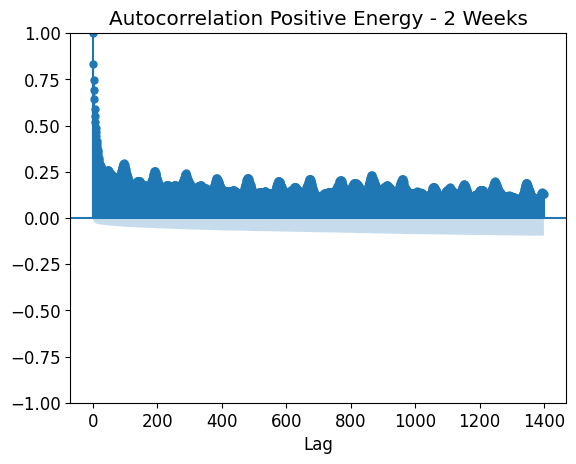
\includegraphics[width=1\linewidth]{pictures/Autocorrelation Positive Energy - 2 Weeks.png}
	\caption{Total Average Positive Energy Price}
	\label{fig:Autocorrelation Positive Energy Price}
\end{figure}

Auch Trends sind in den Daten keine vorhanden. So zeigt die Abbildung \ref{fig:posEngOverview} beispielhaft jeweils 30 Tage aus dem frühen, mittleren und spätem Jahresverlauf.
Auch hier sind weder Trends noch Saisonale entwicklungen zu erkennen.

\begin{figure}[!h]
	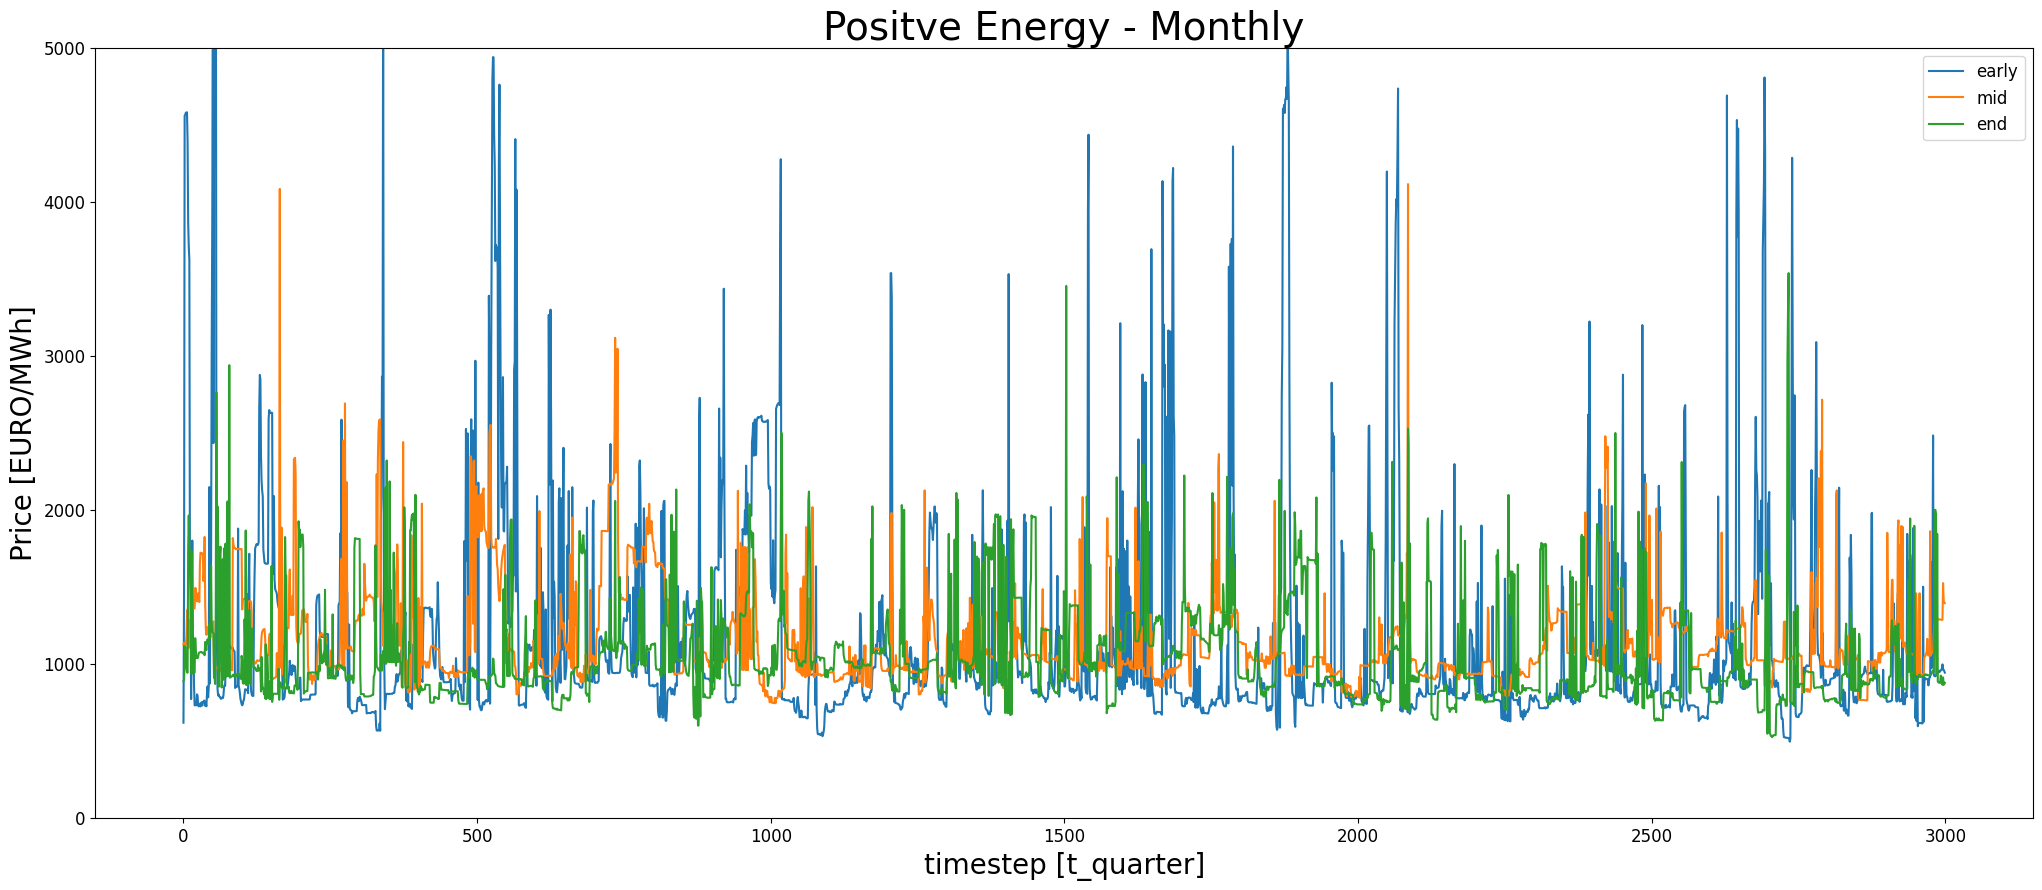
\includegraphics[width=1\linewidth]{pictures/posEngOverview.png}
	\caption{Overview Positive Energy Price}
	\label{fig:posEngOverview}
\end{figure}
\todo{das ist eine grafik mit den alten average preise, mache eine graifk mit den richtigen grenzpreisen}
\todo{grafiken verschiedene Preisszenarien}
\todo{appendix verweis zu python code}

Zu szenario generation werden Realmarkt daten aus dem Jahre 2023 herangezogen.
Das Jahr 2023 wird zuerst hinsichtlich volatilen Energiequellen untersucht [siehe Tabelle \ref{tab:energy_sources_std}].
Hierbei zeigt sich das besonders Solar und Wind Onshore Kraftwerke einer volatilen Produktion unterliegen.

\begin{table}[ht]
	\centering
	\begin{tabular}{|l|r|}
		\hline
		\textbf{Source}                 & \textbf{Standard Deviation} \\
		\hline
		Geothermal                      & 5.956190                    \\
		Fossil Oil                      & 85.360298                   \\
		Waste                           & 133.320136                  \\
		Hydro Water Reservoir           & 167.126363                  \\
		Hydro Run-of-river and poundage & 310.405850                  \\
		Biomass                         & 429.594441                  \\
		Nuclear                         & 1223.169733                 \\
		Hydro Pumped Storage            & 1543.402759                 \\
		Wind Offshore                   & 1833.588012                 \\
		Fossil Gas                      & 2916.794393                 \\
		Fossil Hard coal                & 3364.505964                 \\
		Fossil Brown coal/Lignite       & 3799.694920                 \\
		Solar                           & 9879.907341                 \\
		Wind Onshore                    & 10506.831136                \\
		\hline
	\end{tabular}
	\caption{Standard deviation per energy generator type}
	\label{tab:energy_sources_std}
\end{table}

Anschließend wird die summierte Produktion von Solar und Wind Onshore je Zeitpunkt berchnet und
durch die gesamte Produktion aller Kraftwerke zum gleichen Zeitpunkt geteilt. So erzielen wir den relativen
Anteil dieser besonders volatilen Kraftwerke an der gesamten Produktion. Die These ist nun das wenn ein Vorhersagefehler eintritt
dieser besonders starke Auswirkungen hat, da er einen größeren Anteil an der Gesamtproduktion betrifft.
Diese relativen Produktionsdaten volatiler Kraftwerke werden nun in 36 Quantile eingeteilt. Das erste, mittlere und letzten
Quantil werden nun zur Szenariogeneration benutzt.

Hierfür werden die Zeitpunkte der Quantile, die auf stündlichen Daten beruhen, auf einen viertelstündlichen rythmus extrapoliert und
dazugehörigen Regelarbeitsmarkt daten vom betreffenden Zeitabschnit exportiert.

So ergeben sich 10 mögliche Szenarien für Tage mit hoher, mittlerer und niedrigem Anteil einer volatilem Produktion.

Abbildung   bis
\todo{abbildungen ergänzen}
zeigt nun das zwar das allgemeine Preisniveau steigt, aber da man mit dem hohen Anteil erneuerbarer Energien
kalkuliert und somit auf die hohe volatilität eingeplant ist halten sich ansonsten die Auswirkugen in grenzen.
Die sehr hohen Ausreißer scheinen sich in den Szenarien zu zeigen in denen man nicht mit all zu hohen außreißern rechnet
und
\todo{den teil drinne lassen?}




-> ziel für das hoch und runter setzten der linie ... -> erklärung was ich damit bezwecken möchte in dem entsprechendem Mark


\textbf{Perfekte Vorraussicht}\\
Die einfachste Methode zur Erstellung von Zeitreihendaten wäre die verwendung von

\textbf{SARIMA}\\

\textbf{TBATS}\\
--> RL
-> ziel für das hoch und runter setzten der linie ... -> erklärung was ich damit bezwecken möchte in dem entsprechendem Mark


-> ziel für das hoch und runter setzten der linie ... -> erklärung was ich damit bezwecken möchte in dem entsprechendem Mark

\textbf{approximierte Linie}
--> DA
\textbf{reale Szenarien}
-> ziel für das hoch und runter setzten der linie ... -> erklärung was ich damit bezwecken möchte in dem entsprechendem Mark

%--> kann über  mondpreis eskapen\\
%--> können eine kaum genutzte szenarioeplosion vermeiden (wording nochmal überarbeiten)\\
%- vereinfachung der RL markt mechanik/restriktionen
%--> stellen über batterie gleichung sicher das wir immer liefer können und vermeiden so komplexe $q_RA$ restriktionen (wann wie wo gelten)\\
%--> wir stellen einfach sicher das wir immer liefern könnten und fertig\\

$\omega_{RA}(s_{RA})$ -> sind gleichverteilt
\subsection{Preis Vorhersagen - genaue Modelierung}
\textbf{RL}
-->appendix
\todo{Python Code appendix verweis}
\textbf{DA}
-->appendix
\todo{Python Code appendix verweis}
\textbf{RA}


Data from ENTSOE transperency platform
\todo{ref entsoe}
-->appendix
\todo{Python Code appendix verweis}


\subsubsection{Augmented Dickey Fuller Test}
\subsubsection{Stationary}
Stationär wenn:
\begin{enumerate}
	\item Mittelwert konst.
	\item Varianz konst.
	\item keine Siasionalität
\end{enumerate}


\subsection{Simplification}

wir betrachten uns als teil eines bieterbundes
Um den rechenaufwand und die komplexität des models zu begrenzen wurden ein paar vereinfachungen vorgenommen.
Diese vereinfachungen beschränken kaum die realitätsnähe des Models.

Nochfolgende eine geordnete Aufführung welche Vereinfachungen getroffen wurden.
\subsubsection{RL}

\subsubsection{DA}
\subsubsection{RA}
\subsubsection{Battery Storage Status}

$Q(s) * p(s) * \omega(s)$\\
Die Daten hierfür lassen sich exemplarisch wie folgt darstellen:\\
\begin{tabular}{c|c|c}
	Szenario $s$ & Preis $p(s)$ & Wahrscheinlichkeit $\omega(s)$ \\
	s1           & 90           & 0.6                            \\
	s2           & 100          & 0.5                            \\
	s3           & 110          & 0.4                            \\
\end{tabular}\\


Dabei repräsentiert die Wahrscheinlichkeit die Chance für einen Zuschlag zum zugeordneten Szenariopreis. Ein Zuschlag bei gegebenem Gebot wird als eintreffen des Szenarios interpretiert. Ein geringerer Gebotspreis führt immer zu einer höheren Zuschlagswahrscheinlichkeit. Die Summe aus der Chance für einen Zuschlag und der Chance für eine Ablehnung ergibt dabei immer 1. Die Äste des Szenariobaums stellen dabei die Unterschiedlichen Preisoptionen dar. Mit einem Mengengebot auf einen bestimmten Preis "aktivieren" wird der entsprechende Teil des Szenariobaums aktiviert. Da die gesamte Menge durch $\sum_s Q(s) \leq r$  restriktiert ist, kann eine einzelne Menge (z.B.: 1 MW) nur einmal vergeben werden. Theoretisch ist es möglich, dass unterschiedliche Mengengebote zu unterschiedlichen Preisszenarien erfolgen. Praktisch errechnet der Algorithmus welcher Ast des Szenariobaums den höchsten Erwartungswert ($w(s)*p(s)$) besitzt und bietet entsprechend die maximale Menge an dieser Stelle. \\

Im ersten Schritt wird die optimale Entscheidung am Regelleistungsmarkt berechnet. Hierfür werden die Erwartungswerte aller möglichen Szenarien ausgerechnet (siehe 1.4).\\

Im zweiten Schritt werden die, vorher errechneten, Ergebnisse (Mengengebote zum entsprechenden Preis) als exogene Parameter in das 2. Modell eingefügt. Es folgt eine Auswertung ob zum entsprechenden Gebot ein Zuschlag erfolgt. Anschließend wird, wie im vorherigen Schritt, die optimale Entscheidung für den Day Ahead Markt bestimmt (siehe 1.4.2).\\

Im letzten Schritt werden die Ergebnisse des Day Ahead Marktes in das 3. Modell integriert. Nachfolgend wird überprüft ob zum entsprechenden Gebot ein Zuschlag erfolgt. Zum Schluss wird die optimale Entscheidung am Regelarbeitsmarkt ermittelt (siehe 1.4.3).\\






\subsubsection{Preisvorhersage}

- verschiedene Methoden ...
-> implementiert in python
-> alle können dem model hinzugefügt werden
-> ich habe dann aus diesen und jenen gründe diese Variante gewählt

Methode - beschreibung
Methode - Implementierung
Methode - Pro cons
Methode - hinweis welcher anhang





Die verschiedenen Preis Szenarien werden mittels SARIMA Analyse exogen errechnet. Die SARIMA Analyse errechnet eine Wahrscheinlichkeitsverteilung (mehr dazu im Abschnitt Preisvorhersage), welche zu jedem Preis dessen Eintrittswahrscheinlichkeit angibt. Zu Vereinfachungszwecken werden die kontinuierlichen Preis-Wahrscheinlichkeits-Pärchen per Szenario Reduktion [N. Growe-Kuska, H. Heitsch, and W. Romisch, “Scenario reduction and scenario tree construction for power management problems,” in Proc.
		2003 IEEE Bologna Power Tech Conf., vol. 3, Jun. 2003, pp. 7.] auf signifikante Szenarion reduziert.
Diese diskreten Preis-Wahrscheinlichkeits-Pärchen werden mathematisch über einen Parameter/Binär-Variablen Kombination abgebildet.\\
\\
\textbf{Beispiel: Umwandlung kontinuierliche Variable zu Diskreter:}
\\
Betrachtet werden folgende diskrete Preis-Wahrscheinlichkeits-Pärchen aus einer beispielhaften Szenarioreduktion:\\
\\
\begin{tabular}{c|c|c}
	Szenario $s_{DA}$ & Preis $p_{DA}(s_{DA})$ & Wahrscheinlichkeit $\omega_{DA}(s_{DA})$ \\
	s1                & 90                     & 0.6                                      \\
	s2                & 100                    & 0.5                                      \\
	s3                & 110                    & 0.4                                      \\
\end{tabular}\\
\\

$P_{DA} * \omega_{DA}(P_{DA}) \rightarrow \sum_{s_{DA}} p_{DA}(s_{DA}) * \omega_{DA}(s_{DA})$\\

\todo{Erklärung mit summe wahrscheinlichkeiten 1}

Hier und im folgenden weggelassen ist jeweils die Gegenwahrscheinlichkeit $1-\omega_{DA}(s_{DA})$ da sie die Ablehnung des Gebots repräsentiert und somit in der Ertragsrechnung mit 0 multipliziert werden würde und entsprechend entfällt.\\
\\

\subsection{Marktmodelle}

Das Modell ist in der Lage an drei Märkten zu bieten. Ein Gebot umfasst immer eine Menge sowie einen dazu gehörigen Preis. Zuerst erfolgt das Gebot am Regelleistungsmarkt, dann am Day Ahead Markt und schließlich das Gebot am Regelarbeitsmarkt.
\todo{Übersicht über zeitlichen Ablauf der einzelnen Märkte}

Dabei ergibt sich der zu maximierende Ertrag wie folgt:

$Ertrag = Menge * Preis$

In der stochastischen Programmierung wird eine Wahrscheinlichkeit hinzugefügt welche angibt wie wahrscheinlich der Zuschlag zum entsprechend gebotenen Preis ist.\\

$Ertrag = Menge * Preis * Wahr(Preis)$\\

In den folgenden Kapiteln werden zuerst die einzelnen Märkte  individuell beschrieben. (siehe 1.3.1 bis 1.3.3).
Nachfolgend wird die Überführung der Einzelmarktprobleme in eine Gesamtentscheidung erläutert.
1.4 skizziert hierfür zuerst die schematische Berechnung der Einzelentscheidungen.
1.4.1 bis 1.4.3 erläutern dann die detaillierten Einzelberechnungen.

\subsubsection{Regelleistungsmarkt}
Für den Regelleistungsmarkt ergibt sich dann die folgende Zielfunktion.\\

$max Profit_{RL} = Q_{RL} * p_{RL} * \omega_{RL}(p_{RL})$

Durch einsetzen der vorhergesagten Preise ergibt sich dann die folgende Gleichung:\\

$max Profit_{RL} = \sum_{s_{RL}} Q_{RL}(s_{RL}) * p_{RL}(s_{RL}) * \omega_{RL}(s_{RL})$\\

Zu beachten ist, dass auch die Menge nun Szenarioabhängig ist, so kann theoretisch auf für jedes angenommene Szenario separat geboten werden. Praktisch ist dies nicht an zu nehmen, da der Algorithmus die höchst mögliche Menge immer dem höchsten Preiserwartungswert  zuordnen wird. Auf diese Weise dient die Menge als abstrakte binäre Aktivierungsvariable der verschiedenen Preisszenarien.
\todo{den Part Menge als abstrakte binäre Aktivierungsvariable eventuell nochmal überarbeiten und entsprechend oben anpassen }
\todo{eventuell binär variable nur an Preis koppeln und das dann anders heraus ziehen}
Für die anschließenden Märkte ist es wichtig zu wissen ob das Gebot angenommen wurde oder nicht. Dies wird über eine binäre Variable $B_{RL}$ repräsentiert.

$max Profit_{RL} = \sum_{s_{RL}} Q_{RL}(s_{RL}) * B_{RL}(s_{RL}) * p_{RL}{RL}(s_{RL}) * \omega_{RL}(s_{RL})$\\
s.t.:\\
$c_{RL} \leq p_{RL}(s_{RL}) + M * B_{RL}(s_{RL}) $\\
$c_{RL} \geq p_{RL}(s_{RL}) - M * (1 - B_{RL}(s_{RL})) $\\
$B_{RL} \in \{0,1\}$\\
$M$ ist hierbei eine sehr große Zahl. Über die Kombination beider Nebenbedingungen wird sicher gestellt, dass der Lösungsalgorithmus die binäre Variable immer so setzt, dass sie dem tatsächlichen Marktresultat entspricht. So entspricht $B_{RL} = 1$ einem angenommenen Gebot und $B_{RL} = 0$ entspricht einem abgelehnten Gebot.\\
\todo{ausführliche Erklärung zusammenspiel Nebenbedingungen und binär Variable}
\todo{Zitat einfügen}




\todo{Zitat einfügen}
Zu beachten ist das sowohl positive als auch negative Leistungsgebote abgegeben werden können. Die vollständige Zielfunktion drückt sich dann wie folgt aus:\\

\begin{center}
	$max_{Q^{in}_{RL}(s_{RL}), Q^{out}_{RL}(s_{RL})} Profit_{RL}$\\
	$=$\\
	$\sum_{s^{in}_{RL}} Q^{in}_{RL}(s_{RL}) * p(s^{in}_{RL}) * \omega_{RL}(s^{in}_{RL}) +$\\
	$\sum_{s^{out}_{RL}} Q^{out}_{RL}(s_{RL}) * p(s^{out}_{RL}) * \omega_{RL}(s^{out}_{RL})$\\
\end{center}


(grundlegende Beschränkungen der Definitionsbereiche:)\\
$B^{in}_{RL}(s^{in}_{RL}),B^{out}_{RL}(s^{out}_{RL}) \in \{0,1\}\quad\forall s^{in}_{RL},s^{out}_{RL} $\\
$Q^{in}_{RL}(s^{in}_{RL}),Q^{out}_{RL}(s^{out}_{RL}) \geq 0\quad\forall  s^{in}_{RL},s^{out}_{RL} $\\
(wird später durch Nebenbedingungen des Regelarbeitsmarktes ersetzt:)\\
$\sum_{s^{in}_{RL}}Q^{in}_{RL}(s^{in}_{RL}),\sum_{s^{out}_{RL}}Q^{out}_{RL}(s^{out}_{RL}) \leq r$\\
$a + \sum_{s^{in}_{RL}}Q^{in}_{RL}(s^{in}_{RL})\geq \sum_{s^{out}_{RL}}Q^{out}_{RL}(s^{out}_{RL}) $\\
\todo{alle gleichungen checken wegen $\forall$}
\todo{alle gleichungen mit nummerierung und beschreibung{?} überarbeiten}

\subsubsection{Day Ahead Markt}
Simultan zu dem vorherigen Kapitel ergeben sich dann dich Gleichungen für den Day Ahead Markt.
Der Day Ahead Markt ist der Markt an dem der Strom des Windparks vermarktet wird. Dementsprechend gibt es keine positiven und negativen Gebote.

\begin{center}
	$max_{Q_{DA}(s_{DA})} Profit_{DA}$\\
	$=$\\
	$\sum_{s_{DA}} Q_{DA}(s_{DA}) * p(s_{DA}) * \omega_{DA}(s_{DA})$\\

\end{center}
s.t.:\\

s.t.:\\
(grundlegende Beschränkungen der Definitionsbereiche:)\\
$Q_{DA}(s_{DA}) \geq 0\quad\forall  s_{DA} $\\
$ \sum_{s_{DA}}Q_{DA}(s_{DA}) \leq capPark $\\
(wird später durch Nebenbedingungen des Regelarbeitsmarktes ergänzt:)\\
$ \sum_{s_{DA}}Q_{DA}(s_{DA})\leq a  $\\
\todo{annahme perfekte Vorraussicht Windpark}


\subsubsection{Regelarbeitsmarkt}
Simultan zum Regelleistungsmarkt ergibt sich der Regelarbeitsmarkt:
\todo{erklärung zusammenhang regelleistungsmarkt regelarbeitsmarkt}
\begin{center}
	$max_{Q^{in}_{RA}(s_{RA}), Q^{out}_{RA}(s_{RA})} Profit_{RA}$\\
	$=$\\
	$\sum_{s^{in}_{RA}} Q^{in}_{RA}(s_{RA}) * p(s^{in}_{RA}) * \omega_{RA}(s^{in}_{RA}) +$\\
	$\sum_{s^{out}_{RA}} Q^{out}_{RA}(s_{RA}) * p(s^{out}_{RA}) * \omega_{RA}(s^{out}_{RA})$\\
\end{center}
s.t.:\\
(grundlegende Beschränkungen der Definitionsbereiche:)\\
$Q^{in}_{RA}(s^{in}_{RA}),Q^{out}_{RA}(s^{out}_{RA}) \geq 0 \quad\forall s^{in}_{RA},s^{out}_{RA} $\\
$Q^{in}_{RA}(s^{in}_{RA}),Q^{out}_{RA}(s^{out}_{RA}) \geq 0\quad\forall  s^{in}_{RA},s^{out}_{RA} $\\


\subsection{Berechnung optimale Einzelentscheidungen}
Um die optimale Erststufenentscheidung zu berechnen wird der Erwartungswert sämtlicher Zweige des Szenario-Baum ausgerechnet.
Die Entscheidung zu welchem Preis am positiven sowie negativen Regelleistungsmarkt geboten werden soll erfolgt zeitgleich.
Daraus ergeben sich 4 Szenarien:
\begin{enumerate}
	\item $RL^{in}$ \& $RL^{out}$ angenommen
	\item nur $RL^{in}$ angenommen
	\item nur $RL^{out}$ angenommen
	\item $RL^{in}$ \& $RL^{out}$ abgelehnt
\end{enumerate}
Es folgt eine systematische Darstellung dieser Rechnung:
\begin{table}


	\begin{tabular}{|c|c|}
		\hline
		Formelzeichen & Erklärung                                       \\
		\hline
		$\omega()$    & Wahrscheinlichkeit für Preis/Mengen Kombination \\
		$E()$         & Ertrag von Preis/Mengen                         \\
		              & Kombination am Markt                            \\
		$RL^{in/out}$ & Preis/Mengen Kombination am Regelleistungsmarkt \\
		$DA$          & Preis/Mengen Kombination am Day Ahead Markt     \\
		$RA^{in/out}$ & Preis/Mengen Kombination am Regelarbeitsmarkt   \\
		\hline
	\end{tabular}
	\caption{table}
	\label{tab:my_label}
\end{table}

\begin{alignat*}{3}
	max Profit =                                                                                                                                               \\
	\sum \sum \omega(RL^{in})* \omega(RL^{out})       & * \Biggl[E(RL^{in}) + E(RL^{out})                                                                      \\
	                                                  & +\sum_{DA} \omega(DA) *           &  & \Biggl(E(DA)                                                    \\
	                                                  &                                   &  & + \sum_{RA^{in}} \omega(RA^{in}) * E(RA^{in})                   \\
	                                                  &                                   &  & + \sum_{RA^{out}} \omega(RA^{out}) * E(RA^{out})\Biggr)         \\
	                                                  & +\sum_{DA} (1- \omega(DA) *       &  & \Biggl(\sum_{RA^{in}} \omega(RA^{in}) * E(RA^{in})              \\
	                                                  &                                   &  & + \sum_{RA^{out}} \omega(RA^{out}) * E(RA^{out})\Biggr) \Biggr] \\
	+\sum \sum (1-\omega(RL^{in})) * \omega(RL^{out}) & * \Biggl[E(RL^{in}) + E(RL^{out})                                                                      \\
	                                                  & +\sum_{DA} \omega(DA) *           &  & \Biggl(E(DA)                                                    \\
	                                                  &                                   &  & + \sum_{RA^{in}} \omega(RA^{in}) * E(RA^{in})                   \\
	                                                  &                                   &  & + \sum_{RA^{out}} \omega(RA^{out}) * E(RA^{out})\Biggr)         \\
	                                                  & +\sum_{DA} (1- \omega(DA)) *      &  & \Biggl(\sum_{RA^{in}} \omega(RA^{in}) * E(RA^{in})              \\
	                                                  &                                   &  & + \sum_{RA^{out}} \omega(RA^{out}) * E(RA^{out})\Biggr) \Biggr] \\
\end{alignat*}
\begin{alignat*}{3}
	+\sum \sum \omega(RL^{in})* (1-\omega(RL^{out}))     & * \Biggl[E(RL^{in}) + E(RL^{out})                                                                       \\
	                                                     & +\sum_{DA} \omega(DA) *           &  & \Biggl(E(DA)                                                     \\
	                                                     &                                   &  & + \sum_{RA^{in}} \omega(RA^{in}) * E(RA^{in})                    \\
	                                                     &                                   &  & + \sum_{RA^{out}} \omega(RA^{out}) * E(RA^{out})\Biggr)          \\
	                                                     & +\sum_{DA} (1- \omega(DA)) *      &  & \Biggl(\sum_{RA^{in}} \omega(RA^{in}) * E(RA^{in})               \\
	                                                     &                                   &  & + \sum_{RA^{out}} \omega(RA^{out}) * E(RA^{out})\Biggr) \Biggr]  \\
	+\sum \sum (1-\omega(RL^{in}))* (1-\omega(RL^{out})) & * \Biggl[E(RL^{in}) + E(RL^{out})                                                                       \\
	                                                     & +\sum_{DA} \omega(DA) *           &  & \Biggl(E(DA)                                                     \\
	                                                     &                                   &  & + \sum_{RA^{in}} \omega(RA^{in}) * E(RA^{in})                    \\
	                                                     &                                   &  & + \sum_{RA^{out}} \omega(RA^{out}) * E(RA^{out})\Biggr)          \\
	                                                     & +\sum_{DA} (1- \omega(DA)) *      &  & \Biggl(\sum_{RA^{in}}\omega(RA^{in}) * E(RA^{in})                \\
	                                                     &                                   &  & + \sum_{RA^{out}} \omega (RA^{out}) * E(RA^{out})\Biggr) \Biggr] \\
\end{alignat*}

\subsubsection{Berechnung optimale Erststufenentscheidungen}

Da die einzelnen Mengen, je nach Szenario, unterschiedlichen Restriktionen unterliegen werden ihnen separate Variablen zugewiesen.
Es folgt eine ausführliche Formel für die Berechnung der optimalen Erststufenentscheidung:
(Die einzelnen Mengen Formelzeichen setzen sich wie folgt zusammen:
\begin{enumerate}
	\item $Q$ - Menge
	\item $Q_{\pmb{y}}$ - am welchem Markt die Menge Geboten wird
	\item $Q^{\pmb{i}}_{y}$ - (nur für die Regelmärkte) welche Art von Leistung geboten wird: negativ$\rightarrow$in / positiv$\rightarrow$out
	\item $Q^{i\pmb{r...}}_{y}$ - welchen Restriktionen die Menge unterliegt, da in vorhergehenden Märkten entsprechende Zuschläge erfolgt sind
\end{enumerate}
Beispiele:
\begin{itemize}
	\item $Q^{outrRL}_{RA}$ - positive Menge am Regelarbeitsmarkt restriktiert durch ein bezuschlagtes Regelleistungsmarkt-Gebot
	\item $Q^{rRL}_{DA}$ - Menge am Day Ahead Markt restriktiert durch ein bezuschlagtes Regelleistungsmarkt-Gebot
	\item $Q^{in}_{RA}$ - negative Menge am Regelarbeitsmarkt mit keinen Restriktionen
\end{itemize}


\begin{alignat*}{3}
	max Profit  =                                                                            &                                                                                                                                                                                          \\
	for\quad accepted\quad RL\quad in \& out:                                                &                                                                                                                                                                                          \\
	\sum_{s^{out}_{RL}}\sum_{s^{in}_{RL}} \omega_{RL}(s^{in}_{RL})*\omega_{RL}(s^{out}_{RL}) & *\Biggl[\tfrac{1}{4} * Q^{in}_{RL} (s^{in}_{RL}) * p(s^{in}_{RL}) &  & +\tfrac{1}{4} *  Q^{out}_{RL}(s^{out}_{RL}) * p(s^{out}_{RL})                                                     \\
	                                                                                         & + \sum_{s_{DA}}\omega_{DA}(s_{DA})                                &  & \Biggl(\tfrac{1}{4}(Q^{rRL}_{DA}(s_{DA}) * p(s_{DA}))                                                             \\
	                                                                                         &                                                                   &  & + \sum_{s^{in}_{RA}} Q^{inrRLDA}_{RA}(s^{in}_{RA}) * p(s^{in}_{RA}) * \omega_{RA}(s^{in}_{RA})                    \\
	                                                                                         &                                                                   &  & + \sum_{s^{out}_{RA}} Q^{outrRLDA}_{RA}(s^{out}_{RA}) * p(s^{out}_{RA}) * \omega_{RA}(s^{out}_{RA})\Biggr)        \\
	                                                                                         & + \sum_{s_{DA}}(1-\omega_{DA}(s_{DA}))                            &  & * \Biggl(\sum_{s^{in}_{RA}} Q^{inrRL}_{RA}(s^{in}_{RA}) * p(s^{in}_{RA}) *             \omega_{RA}(s^{in}_{RA})   \\
	                                                                                         &                                                                   &  & + \sum_{s^{out}_{RA}} Q^{outrRL}_{RA}(s^{out}_{RA}) * p(s^{out}_{RA}) * \omega_{RA}(s^{out}_{RA}) \Biggr) \Biggr] \\
\end{alignat*}
for accepted RL in 	\& declined out:\\
\begin{alignat*}{3}
	+\sum_{s^{out}_{RL}}\sum_{s^{in}_{RL}} \omega_{RL}(s^{in}_{RL})*(1-\omega_{RL}(s^{out}_{RL})) * & \Biggl[Q^{in}_{RL}(s^{in}_{RL}) * p(s^{in}_{RL}) &  &                                                                                                              \\
	                                                                                                & + \sum_{s_{DA}}\omega_{DA}(s_{DA}) *             &  & \Biggl(Q^{rRL}_{DA}(s_{DA}) * p(s_{DA})                                                                      \\
	                                                                                                &                                                  &  & + \sum_{s^{in}_{RA}} Q^{inrRLDA}_{RA}(s^{in}_{RA}) * p(s^{in}_{RA}) * \omega_{RA}(s^{in}_{RA})               \\
	                                                                                                &                                                  &  & + \sum_{s^{out}_{RA}} Q^{outrDA}_{RA}(s^{out}_{RA}) * p(s^{out}_{RA}) * \omega_{RA}(s^{out}_{RA})\Biggr)     \\
	                                                                                                & + \sum_{s_{DA}}(1-\omega_{DA}(s_{DA}))           &  &                                                                                                              \\
	                                                                                                &                                                  &  & * \Biggl( \sum_{s^{in}_{RA}} Q^{inrRL}_{RA}(s^{in}_{RA}) * p(s^{in}_{RA}) * \omega_{RA}(s^{in}_{RA})         \\
	                                                                                                &                                                  &  & + \sum_{s^{out}_{RA}} Q^{out}_{RA}(s^{out}_{RA}) * p(s^{out}_{RA}) * \omega_{RA}(s^{out}_{RA})\Biggr)\Biggr]
\end{alignat*}
for declined RL in\& accepted out:\\
\begin{alignat*}{3}
	+\sum_{s^{out}_{RL}}\sum_{s^{in}_{RL}}(1-\omega_{RL}(s^{in}_{RL}))*\omega_{RL}(s^{out}_{RL})* & \Biggl[Q^{out}_{RL}(s^{out}_{RL}) * p(s^{out}_{RL}) &  &                                                                                                                  \\
	                                                                                              & + \sum_{s_{DA}}\omega_{DA}(s_{DA})                  &  & * \Biggl(Q^{rRL}_{DA}(s_{DA}) * p(s_{DA})                                                                        \\
	                                                                                              &                                                     &  & + \sum_{s^{in}_{RA}} Q^{inrDA}_{RA}(s^{in}_{RA}) * p(s^{in}_{RA}) * \omega_{RA}(s^{in}_{RA})                     \\
	                                                                                              &                                                     &  & + \sum_{s^{out}_{RA}} Q^{outrRLDA}_{RA}(s^{out}_{RA}) * p(s^{out}_{RA}) * \omega_{RA}(s^{out}_{RA})\Biggr)       \\
	                                                                                              & + \sum_{s_{DA}}(1-\omega_{DA}(s_{DA}))              &  &                                                                                                                  \\
	                                                                                              &                                                     &  & * \Biggl(\sum_{s^{in}_{RA}} Q^{in}_{RA}(s^{in}_{RA}) * p(s^{in}_{RA}) * \omega_{RA}(s^{in}_{RA})                 \\
	                                                                                              &                                                     &  & + \sum_{s^{out}_{RA}} Q^{outrRL}_{RA}(s^{out}_{RA}) * p(s^{out}_{RA}) * \omega_{RA}(s^{out}_{RA})\Biggr) \Biggr]
\end{alignat*}
for declined RL in\& out:\\
\begin{alignat*}{3}
	+\sum_{s^{out}_{RL}}\sum_{s^{in}_{RL}} (1-\omega_{RL}(s^{in}_{RL}))*(1-\omega_{RL}(s^{out}_{RL})) & *\Biggl[\sum_{s_{DA}}\omega_{DA}(s_{DA}) &  & *\Biggl(Q_{DA}(s_{DA}) * p(s_{DA})                                                                            \\
	                                                                                                  &                                          &  & + \sum_{s^{in}_{RA}} Q^{inrDA}_{RA}(s^{in}_{RA}) * p(s^{in}_{RA}) * \omega_{RA}(s^{in}_{RA})                  \\
	                                                                                                  &                                          &  & + \sum_{s^{out}_{RA}} Q^{outrDA}_{RA}(s^{out}_{RA}) * p(s^{out}_{RA}) * \omega_{RA}(s^{out}_{RA})\Biggr)      \\
	                                                                                                  & + \sum_{s_{DA}}(1-\omega_{DA}(s_{DA}))   &  &                                                                                                               \\
	                                                                                                  &                                          &  & * \Biggl(\sum_{s^{in}_{RA}} Q^{in}_{RA}(s^{in}_{RA}) * p(s^{in}_{RA}) * \omega_{RA}(s^{in}_{RA})              \\
	                                                                                                  &                                          &  & + \sum_{s^{out}_{RA}} Q^{out}_{RA}(s^{out}_{RA}) * p(s^{out}_{RA}) * \omega_{RA}(s^{out}_{RA})\Biggr) \Biggr]
\end{alignat*}




\textbf{Nebenbedingungen}\\
$ Q_{DA} \leq capPark$
Anschlusspunkt:\\
$a + Q^{in}_{RA} \geq Q^{outrRLDA}_{RA} + Q^{rRL}_{DA}$ \\
$a + Q^{in}_{RA} \geq Q^{outrDA}_{RA} + Q_{DA}$ \\
$a + Q^{in}_{RA} \geq Q^{out}_{RA}$ \\
Batterie Restriktionen:\\
$Q^{out}_{RL}, Q^{in}_{RL}, Q^{out}_{RA}, Q^{in}_{RA}, Q^{outrRL}_{RA}, Q^{inrRL}_{RA}, Q^{outrDA}_{RA}, Q^{inrDA}_{RA}, Q^{outrRLDA}_{RA}, Q^{inrRLDA}_{RA} \leq r$\\
Markt Restriktionen:\\
$\sum_{s^{out}_{RA}} Q^{outrRL}_{RA} \geq \sum_{s^{out}_{RL}} Q^{out}_{RL} $\\
$\sum_{s^{in}_{RA}} Q^{inrRL}_{RA} \geq \sum_{s^{in}_{RL}} Q^{in}_{RL} $\\
$\sum_{s^{out}_{RA}} Q^{outrRLDA}_{RA} \geq \sum_{s^{out}_{RL}} Q^{out}_{RL} $\\
$\sum_{s^{in}_{RA}} Q^{inrRLDA}_{RA} \geq \sum_{s^{in}_{RL}} Q^{in}_{RL} $\\




\subsubsection{Berechnung optimale Zweitstufenentscheidung}
Die vorher berechneten optimalen Gebotsmengen $q^{in^*}_{RL}$ \& $q^{out^*}_{RL}$ und Preise $p(s^{out}_{RL})$ \& $p(s^{in}_{RL})$  werden nun exogen in das Modell eingespeist. Sie werden mit einer binären Variable gekoppelt welche angibt ob zum entsprechenden Preis ein Zuschlag erfolgt. Die korrekte Setzung der binären Variable wird über eine Kombination aus 2 Nebenbedingungen sicher gestellt.\\
Schematisch stellt sich dies dann wie folgt dar:\\
$\sum_s q^*(s) * p(s) * B(s)$\\
s.t.:\\
$c \leq p(s) + M * B(s)\quad\forall s $ \\
$c \geq p(s) - M * (1 - B(s))\quad\forall s $ \\

\begin{tabular}{c|c}
	$c$    & Clearing Preis Markt                                                 \\
	$p(s)$ & Gebotspreis für Szenario s                                           \\
	$M$    & sehr große Zahl                                                      \\
	$B(s)$ & binäre Variable welche angibt ob Szenariopreis zuschlag erhalten hat \\
\end{tabular}\\

Das gesamte Modell für den Day Ahead Markt ergibt sich dann wie folgt dar:
\begin{alignat*}{3}
	max Profit  =                  &                                                                                                                                                             \\
	q^{in^*}_{RL} (s^{in}_{RL})    & * p(s^{in}_{RL}) * B^{in}_{RL} (s_{RL})                                                                                                                     \\
	+ q^{out^*}_{RL}(s^{out}_{RL}) & * p(s^{out}_{RL}) * B^{out}_{RL} (s_{RL})                                                                                                                   \\
	                               & + \sum_{s_{DA}}\omega_{DA}(s_{DA})        &  & * \Biggl(Q_{DA}(s_{DA}) * p(s_{DA})                                                                          \\
	                               &                                           &  & + \sum_{s^{in}_{RA}} Q^{inrDA}_{RA}(s^{in}_{RA}) * p(s^{in}_{RA}) * \omega_{RA}(s^{in}_{RA})                 \\
	                               &                                           &  & + \sum_{s^{out}_{RA}} Q^{outrDA}_{RA}(s^{out}_{RA}) * p(s^{out}_{RA}) * \omega_{RA}(s^{out}_{RA})\Biggr)     \\
	                               & + \sum_{s_{DA}}(1-\omega_{DA}(s_{DA}))    &  & * \Biggl(\sum_{s^{in}_{RA}} Q^{in}_{RA}(s^{in}_{RA}) * p(s^{in}_{RA}) *             \omega_{RA}(s^{in}_{RA}) \\
	                               &                                           &  & + \sum_{s^{out}_{RA}} Q^{out}_{RA}(s^{out}_{RA}) * p(s^{out}_{RA}) * \omega_{RA}(s^{out}_{RA}) \Biggr)       \\
\end{alignat*}



\textbf{Nebenbedingungen}\\
Anschlusspunkt:\\
$a + Q^{in}_{RA} \geq Q^{outrRLDA}_{RA} + Q^{rRL}_{DA}$ \\
$a + Q^{in}_{RA} \geq Q^{outrDA}_{RA} + Q_{DA}$ \\
$a + Q^{in}_{RA} \geq Q^{out}_{RA}$ \\
Batterie Restriktionen:\\
$Q^{out}_{RA}, Q^{in}_{RA}, Q^{outrRL}_{RA}, Q^{inrRL}_{RA}, Q^{outrDA}_{RA}, Q^{inrDA}_{RA}, Q^{outrRLDA}_{RA}, Q^{inrRLDA}_{RA} \leq r$\\
Markt Restriktionen:\\
$Q^{out}_{RA} \geq q^{out^*}_{RL} (s^{out}_{RL}) * B^{out}_{RL} (s^{out}_{RL}) $\\
$Q^{in}_{RA} \geq q^{in^*}_{RL} (s^{in}_{RL}) * B^{in}_{RL} (s^{in}_{RL}) $\\
$Q^{outrRL}_{RA} \geq q^{out^*}_{RL} (s^{out}_{RL}) * B^{out}_{RL} (s^{out}_{RL}) $\\
$Q^{inrRL}_{RA} \geq q^{in^*}_{RL} (s^{in}_{RL}) * B^{in}_{RL} (s^{in}_{RL}) $\\
$Q^{outrDA}_{RA} \geq q^{out^*}_{RL} (s^{out}_{RL}) * B^{out}_{RL} (s^{out}_{RL}) $\\
$Q^{inrDA}_{RA} \geq q^{in^*}_{RL} (s^{in}_{RL}) * B^{in}_{RL} (s^{in}_{RL}) $\\
$Q^{outrRLDA}_{RA} \geq q^{out^*}_{RL} (s^{out}_{RL}) * B^{out}_{RL} (s^{out}_{RL}) $\\
$Q^{inrRLDA}_{RA} \geq q^{in^*}_{RL} (s^{in}_{RL}) * B^{in}_{RL} (s^{in}_{RL}) $\\
Modell Restriktionen:\\
(Angenommene/Abgelehnte Gebote)\\
$c^{in}_{RL} \leq p(s^{in}_{RL}) + M * B^{in}_{RL}(s^{in}_{RL})\quad\forall s^{in}_{RL} $ \\
$c^{in}_{RL} \geq p(s^{in}_{RL}) - M * (1 - B^{in}_{RL}(s^{in}_{RL}))\quad\forall s^{in}_{RL} $ \\
$c^{out}_{RL} \leq p(s^{out}_{RL}) + M * B^{out}_{RL}(s^{out}_{RL})\quad\forall s^{out}_{RL} $ \\
$c^{out}_{RL} \geq p(s^{out}_{RL}) - M * (1 - B^{out}_{RL}(s^{out}_{RL}))\quad\forall s^{out}_{RL} $ \\




\subsubsection{Berechnung optimale Drittstufenentscheidung}
Die optimalen 1. und 2. Stufenentscheidungen werden eingefügt. Simultan zum vorherigen Schritt werden sie mit binären Variablen kombiniert die das eintreffen der verschiedenen Szenarien (Gebotsannahme/-ablehnung) signalisieren.
\begin{alignat*}{3}
	max Profit  =                             &                                                                                                \\
	for\quad accepted\quad RL\quad in \& out: &                                                                                                \\
	                                          & q^{in^*}_{RL} (s^{in}_{RL}) * p(s^{in}_{RL}) * B^{in}_{RL} (s_{RL})                            \\
	                                          & + q^{out^*}_{RL}(s^{in}_{RL}) * p(s^{out}_{RL}) * B^{out}_{RL} (s_{RL})                        \\
	                                          & + q^*_{DA}(s_{DA}) * p_{DA}(s_{DA}) * B_{DA}(s_{DA})                                           \\
	                                          & + \sum_{s^{in}_{RA}} Q^{in}_{RA}(s^{in}_{RA}) * p(s^{in}_{RA}) * \omega_{RA}(s^{in}_{RA})      \\
	                                          & + \sum_{s^{out}_{RA}} Q^{out}_{RA}(s^{out}_{RA}) * p(s^{out}_{RA}) * \omega_{RA}(s^{out}_{RA}) \\
\end{alignat*}





\textbf{Nebenbedingungen}\\
Anschlusspunkt:\\
$a + \sum_{s^{in}_{RA}} q^{in^*}_{RA} \geq Q^{out}_{RA} + \sum_{s^{out}_{RA}}(q^{out^*}_{DA} * B^{out}_{DA})$ \\
Batterie Restriktionen:\\
$Q^{out}_{RA}, Q^{in}_{RA}, Q^{outrRL}_{RA}, Q^{inrRL}_{RA}, Q^{outrDA}_{RA}, Q^{inrDA}_{RA}, Q^{outrRLDA}_{RA}, Q^{inrRLDA}_{RA} \leq r$\\
Markt Restriktionen:\\
$Q^{out}_{RA} \geq q^{out^*}_{RL} (s^{out}_{RL}) * B^{out}_{RL} (s^{out}_{RL}) $\\
$Q^{in}_{RA} \geq q^{in^*}_{RL} (s^{in}_{RL}) * B^{in}_{RL} (s^{in}_{RL}) $\\

(Angenommene/Abgelehnte Gebote)\\
$c^{in}_{RL} \leq p(s^{in}_{RL}) + M * B^{in}_{RL}(s^{in}_{RL})\quad\forall s^{in}_{RL} $ \\
$c^{in}_{RL} \geq p(s^{in}_{RL}) - M * (1 - B^{in}_{RL}(s^{in}_{RL}))\quad\forall s^{in}_{RL} $ \\
$c^{out}_{RL} \leq p(s^{out}_{RL}) + M * B^{out}_{RL}(s^{out}_{RL})\quad\forall s^{out}_{RL} $ \\
$c^{out}_{RL} \geq p(s^{out}_{RL}) - M * (1 - B^{out}_{RL}(s^{out}_{RL}))\quad\forall s^{out}_{RL} $ \\
$c_{DA} \leq p(s_{DA}) + M * B_{DA}(s_{DA})\quad\forall s_{DA} $ \\
$c_{DA} \geq p(s_{DA}) - M * (1 - B_{DA}(s_{DA}))\quad\forall s_{DA} $ \\

